
%\begin{savequote}[6cm]
%<< truc
%\qauthor{Test}
%\end{savequote}

\chapter{Caractérisation des architectures NUMA}\label{chap:contrib:characterization}
\chaptertoc

Les chapitres précédents ont décrit l'existant en terme de matériel et de logiciel.
Ce chapitre va se concentrer sur l'analyse et la caractérisation des architectures NUMA et de l'exécution d'application sur celles-ci.
La première section fait la description d'un outil, \outil, que nous avons développé dans le but de faciliter cette opération.
La section~\ref{sec:contribs:machines} fait une description et une étude, à l'aide de \outil, des deux machines expérimentales que nous avons utilisées dans nos expériences.
La section~\ref{sec:contribs:apps:cholesky} montre l'utilisation de \outil sur une étude de cas~: la factorisation de Cholesky.
L'objectif de ce chapitre est de dégager un axe d'amélioration possible du support exécutif à partir des constats fait sur les applications et les machines.

\section{Exécution précise de noyaux}\label{sec:contribs:outil}

Cette partie se concentre sur la présentation de \outil, un outil que nous avons créé afin de faciliter la réalisation d'expériences avec un contrôle précis sur le placement de noyaux à exécuter ainsi que leurs données.
Le but de ces expériences est d'analyser le comportement des parties de calcul critiques aux performances d'une application, sur une architecture donnée.

\subsection{Besoins pour un outil spécifique: \outil}

Il est en général assez facile d'étudier le comportement global d'une application, et d'observer les variations de ce comportement lorsqu'on change certains détails dans l'exécution, comme par exemple via l'utilisation de \emph{numactl}.

En revanche, si l'on connait bien son application, on a envie de pouvoir étudier le comportement précis de certaines de ses parties critiques afin de pouvoir identifier ce qui cause son comportement global.

La suite naturelle de cette identification est de déterminer s'il existe des améliorations possibles pour ce comportement local, et comment l'améliorer en pratique.

Dans le cas d'une application à base de flots de données, chaque partie de l'application est bien identifiée, et correspond à un nœud dans le graphe de tâches.
Toutes les données manipulées par une partie de l'application sont facilement identifiées également, puisqu'il s'agit des connexions entre les nœuds du graphe de tâches.

Dans le contexte d'une machine NUMA, le temps d'exécution d'une tâche dépend à la fois du placement de son exécution, ainsi que du placement de ces données. On a donc envie de pouvoir étudier le comportement individuel de chaque type de tâche en fonction de son placement et du placement des données qu'elle accède.
Une fois cela fait, cela permettra d'identifier des potentielles variations de comportement, et ajuster les heuristiques d'ordonnancement pour prendre en compte ces variations.

Nous n'avons pas trouvé d'outil existant répondant précisément à ce besoin.
BOAST~\cite{Videau2017} est un outil assez proche dans la thématique d'optimisation de noyaux applicatif~: l'utilisateur fourni des noyaux et un ensemble d'optimisations possibles, BOAST en déduit un espace à explorer et va rechercher automatiquement les paramètres optimaux.

Dans notre cas l'objectif n'est pas d'optimiser le code, mais de replacer le noyau applicatif dans une série de situations se présentant au cours de l'exécution réelle de l'application, afin de déterminer des stratégies d'ordonnancement qui pourrait favoriser l'exécution de ce noyau applicatif dans de bonnes conditions.
De fait nous avions également besoin d'un outil qui nous permette de contrôler et faire varier le placement des noyaux et de ses données sur la topologie de la machine, et qui permette une exécution simultanée de noyaux applicatifs.

C'est à ce besoin que répond \outil : une fois que l'utilisateur a isolé les parties critiques de son application, \outil lui permet de définir lesquelles il souhaite exécuter et où, et lui garantir cette exécution, avec un certain nombre de variables observables.

Dans la suite de ce chapitre, on appellera l'ensemble des paramètres décrivant cette expérience un \emph{scenario}.

\subsection{Description d'un scenario}

Ce que l'on appelle ici un \emph{scenario} n'est ni plus ni moins que la description d'une expérience.
Par exemple on pourrait vouloir "observer les performances en gigaflops d'une multiplication de matrices carrées sur le cœur 0 d'une machine".
C'est un scénario simple, et l'exemple que l'on prendra pour illustrer les points un peu plus formel qui vont suivre.

En pratique un scénario est défini par les éléments suivants :
\begin{itemize}
 \item Un ensemble de données et variables~;
 \item Une liste d'actions à effectuer~;
 \item Un ensemble de caractéristiques à observer.
\end{itemize}


Il est important que le format de description d'un scénario soit humainement lisible, et ne conduise pas à une recompilation systématique du programme. C'est donc une description en YAML~\cite{YAML} qui a été choisie.


\paragraph{Modèle d'exécution.}

Le flot d'exécution est le suivant~:
Dans un premier \outil commence par charger le scénario fourni par l'utilisateur, créer les différentes données, et analyser les actions pour déterminer l'ensemble des cœurs physiques qui seront utilisés au cours des actions.
Pour chacun des cœurs utilisés, un thread est créé et attaché à ce cœur. De plus, une file d'actions (FIFO) est créée pour ce thread.
Les actions sont poussées dans les files d'actions correspondantes, dans l'ordre du fichier.
Une fois l'ensemble des actions chargées, les threads exécutent chacun les actions présentes dans leur file, et vont déclencher les mesures de chaque paramètre observé avant et après chaque action.

Une unique primitive de synchronisation est disponible, sous la forme d'une action prédéfinie à insérer dans le scénario~: une barrière sur un ensemble arbitraire de cœurs.


L'architecture de l'outil est donc simple, avec peu de logique relative au contrôle de l'exécution des tâches et à la synchronisation, ce qui permet de minimiser le <<bruit>> lors des expériences.

Les sections suivantes reviennent sur les différentes caractéristiques définissant un scénario, avec des exemples concrets d'utilisation.


\subsubsection{Données et variables}

Elles sont indispensables car c'est là-dessus que vont se baser les actions du scénario.

L'utilisateur doit fournir les noms et types des variables utilisées en paramètre des différents noyaux, elles peuvent être réutilisées par différents noyaux.

\outil ne prend pas en charge l'allocation ou l'initialisation des données. Dans le cas de variables simples comme des constantes, elles peuvent être directement affectées dans le scénario. Dans le cas de variables complexes, l'utilisateur doit déclarer une action d'initialisation (avec ses paramètres) dans \outil, pour pouvoir l'utiliser ensuite dans le scénario pour initialiser les données.
Cette action peut être soit une fonction implémentée comme un module de \outil, soit être un point d'entrée dans une bibliothèque externe.

\outil met néanmoins à disposition une fonction d'allocation ne faisant aucune réutilisation de page, avec une politique explicite d'allocation physique des pages en \emph{first-touch}.


Pour revenir à l'exemple du scénario simple ou l'on souhaite exécuter une multiplication de matrices carrées - |dgemm| - sur un cœur donné, nous avons besoin de trois matrices |a|, |b|, et |c|, ainsi qu'une largeur en nombre d'éléments pour les matrices manipulées, |size|.

Voici concrètement à quoi ressemblerait la déclaration de ces données :

\begin{lstlisting}[language=yaml,caption=Exemple de déclaration de variables,label=lst:tool:data-example]
data:
  - a:
    - type: "double *"
  - b:
    - type: "double *"
  - c:
    - type: "double *"
  - size:
    - type: "int"
    - value: 256
\end{lstlisting}

Nous pouvons voir ici que |size| est initialisée directement, mais les pointeurs |a|, |b|, et |c| seront initialisés plus tard par une action.

\paragraph{Déclarations multiples.}

Il est possible de créer un ensemble de variables en se basant sur un modèle paramétré de nom.
Un nom de variable peut contenir un ensemble de caractères (|[a-zA-Z]+|) encadré par des chevrons (|<>|).
Cet ensemble de caractères est interprété comme un paramètre du nom de la variable, et la déclaration devra alors contenir l'ensemble des valeurs que ce paramètre peut prendre.
L'ensemble des valeurs est soit~: un ensemble d'entier désignant, à la manière d'une boucle, les limites de l'espace d'itération sous la forme |[début, fin, pas]|~; ou bien un ensemble de chaines de caractères qui seront substituées dans le nom de la variable.

L'exemple suivant illustre cette syntaxe en déclarant les variables |a0|, |a2|, |a4|, |a6|, |array_input|, et |array_output|~:

\begin{lstlisting}[language=yaml,caption=Exemple de déclaration de variables paramètrées,label=lst:tool:data-example-for]
data:
  a<i>:
    i: [0, 7, 2]
    type: "double *"
  array_<name>:
    name: ["input", "output"]
    type: "int *"
\end{lstlisting}



\subsubsection{Actions}

C'est là où l'utilisateur décrit effectivement les noyaux exécutés au cours du scénario.
Il indique une série d'actions à exécuter, et avec quels paramètres.

\paragraph{Définition d'une action.}

Les actions peuvent être prédéfinies par \outil, ou encore être implémentées par l'utilisateur comme un module de \outil, ou finalement être un point d'entrée dans une bibliothèque.
Le listing~\ref{lst:tool:declare-action} donne un exemple d'une définition d'action qui serait externe à \outil, où l'on ciblerait la fonction |cblas_dsyrk| de la bibliothèque OpenBLAS.

\begin{figure}[h!]
\begin{lstlisting}[language=yaml,caption=Exemple de définition d'une action externe,label=lst:tool:declare-action]
declare_actions:
  - library: "openblas"
    # Identifiant de l'action
    name: "dsyrk"
    # Point d'entrée dans la bibliothèque
    entry_point: "cblas_dsyrk"
    params:
    - "int"
    - "int"
    - "int"
    - "int"
    - "int"
    - "double"
    - "double *"
    - "int"
    - "double"
    - "double *"
    - "int"
\end{lstlisting}
\end{figure}

\paragraph{Utilisation dans un scénario.}

Un scénario doit contenir une entrée |actions|, qui est le tableau d'actions à réaliser au cours du scénario.
Chaque action peut avoir les caractéristiques suivantes :
\begin{description}
  \item [kernel~:] chaine de caractères identifiant l'action.
    Cet attribut n'a pas de valeur par défaut et est obligatoire.
  \item [core~:] nombre entier indiquant le cœur sur lequel exécuter l'action. Il n'a pas de valeur par défaut, et est obligatoire.
  \item [params~:] liste de variables à passer en paramètre de l'action, leur nom doit correspondre à des données déclarées dans la section précédente.
  \item [repeat~:] nombre entier indiquant le nombre de fois que cette action doit être répétée. La valeur par défaut est 1.
\end{description}

\outil dispose d'une action prédéfinie~: la barrière. Son identifiant est |barrier|, et pour cette action spécifiquement le traitement de l'attribut |core| est un peu différent~: il peut ne pas être spécifié, et auquel cas la barrière sera effectuée sur l'ensemble des cœurs, mais il peut également être un ensemble de cœurs pour restreindre la portée de la barrière.


Si on continue à décrire l'exemple simple d'une multiplication de matrices carrées, il faut que l'on effectue les actions suivantes : l'initialisation de chaque matrice (via une action |init_blas_bloc|, implémentée au préalable par l'utilisateur dans \outil, qui prend en paramètre un pointeur et une largeur de matrice), et le lancement du dgemm une fois que ces matrices sont initialisées.
Afin d'avoir une mesure plus précise du comportement du noyau, on peut indiquer une répétition du noyau, ici on choisit 50 pour l'exemple.

Le listing~\ref{lst:tool:actions-example} montre un exemple réalisant ce scénario.

\begin{figure}[h!]
\begin{lstlisting}[language=yaml,caption=Exemple d'actions à réaliser pour une multiplication de matrice,label=lst:tool:actions-example]
actions:
  - kernel: init_blas_bloc
    params:
    - a
    - size
    core: 0
  - kernel: init_blas_bloc
    params:
    - b
    - size
    core: 0
  - kernel: init_blas_bloc
    params:
    - c
    - size
    core: 0
  - kernel: dgemm
    params:
    - a
    - b
    - c
    - size
    core: 0
    repeat: 50
\end{lstlisting}
\end{figure}

Ici les trois initialisations et le calcul ont lieu sur le même cœur, et sont déroulés dans l'ordre de création, il n'y a donc pas lieu d'utiliser une synchronisation.

\paragraph{Actions paramétrées}

De manière similaire à la déclaration de données, il est possible de paramétrer les actions.
Cela peut être particulièrement pratique dans le cas où l'on souhaite observer l'exécution concurrente de plusieurs noyaux de calcul.

Cela se fait à l'aide d'une action spéciale \emph{for}, qui doit définir plusieurs attributs~: |var|, qui contient le nom de la variable d'itération, et |actions|, qui contient la liste des actions à effectuer.
Pour définir l'espace d'itération, l'utilisateur doit spécifier un et un seul des deux attributs suivants~: |limits|, qui s'exprime sous la forme |[débug, fin, pas]| et permet d'exprimer les limites de la boucles~; ou |values|, qui indique une liste explicite des valeurs que peut prendre la variable.

Le listing~\ref{lst:tool:actions-example-sync} fait une utilisation de cette syntaxe pour exécuter 4 dgemm simultanément sur les cœurs 0, 1, 2, et 3, en ayant au préalable initialisé les données nécessaires.

\begin{figure}[h!]
\begin{lstlisting}[language=yaml,caption=Exemple de déclaration d'actions synchronisées,label=lst:tool:actions-example-sync]
data:
  # Déclaration de a0, a1, a2, a3, etc
  a<i>:
    i: [0, 3, 1]
    type: "double *"
  b<i>:
    i: [0, 3, 1]
    type: "double *"
  c<i>:
    i: [0, 3, 1]
    type: "double *"
actions:
  # Initialise a0, b0, et c0 sur le coeur 0,
  # a1, b1, et c1 sur le coeur 1, etc.
  - for:
      var: name
      values: ["a", "b", "c"]
      actions:
        - for:
            var: i
            limits: [0, 3, 1]
            actions:
              - kernel: init_blas_bloc
                params:
                - <name><i>
                - size
                core: <i>
  # Synchronisation avant de lancer les dgemm
  - kernel: barrier
  # Lancement d'un dgemm sur le coeur 0 utilisant a0, b0, et c0,
  # et d'un dgemm sur le coeur 1 utilisant a1, b1, et c1, etc.
  - for:
      var: i
      limits: [0, 3, 1]
      actions:
        - kernel: dgemm
          params:
          - a<i>
          - b<i>
          - c<i>
          - size
          core: <i>
          repeat: 50
\end{lstlisting}
\end{figure}

Cette syntaxe permet d'exprimer des scénarios relativement complexe de manière compacte.
En revanche simplement exécuter ces actions ne nous donnera pas grand chose, il faut donc définir un ensemble de caractéristiques à observer pendant leur exécution.

\subsubsection{Observateurs}

\outil utilise des \emph{Observateurs} pour enregistrer certaines caractéristiques au cours de la vie du programme.
Un observateur peut avoir plusieurs attributs~:
\begin{description}
  \item [name~:] un identifiant d'observateur existant dans \outil.
  \item [params~:] les paramètres à passer lors de la création de l'observateur.
  \item [kernels~:] une liste d'identifiants d'actions sur lesquelles appliquer cet observateur.
\end{description}

\outil propose de base deux observateurs élémentaires~:

\begin{itemize}
  \item \emph{time}~: le temps passé dans l'action (en millisecondes).
  \item \emph{papi}~: permettant de relever des compteurs de performances à travers PAPI.
\end{itemize}

L'utilisateur peut implémenter lui-même des observateurs additionnels au sein de \outil.
Dans notre cas nous avons implémenté des observateurs spécifiques à certains noyaux d'algèbre linéaire, qui dérivent du temps passé dans l'action et qui indique la performance équivalente en Gflops.

La figure~\ref{lst:tool:watchers-example} illustre à quoi ressemblerait la section du scénario si nous souhaitions observer la performance de dgemm en Gflops, le nombre de cycles, ainsi que le nombre de \emph{cache miss} de niveau 3 pendant l'exécution de chaque dgemm.

\begin{figure}[h!]
\begin{lstlisting}[language=yaml,caption=Exemple de déclaration d'observateurs,label=lst:tool:watchers-example]
watchers:
  - name: flops_dgemm
    # Le nombre de flops dépend de la taille de la matrice,
    # qu'il faut donc donner en paramètre.
    params:
      - size
    kernels:
      - dgemm
  - name: papi
    params:
      - PAPI_TOT_CYC
      - PAPI_L3_TCM
    kernels:
      - dgemm
\end{lstlisting}
\end{figure}

L'ensemble des compteurs à observer étant passé tel quel à PAPI, il est donc de la responsabilité de l'utilisateur de fournir un ensemble de compteurs compatibles entre eux.

L'observation se faisant sur la base d'une seule action, une ligne récapitulative est générée à partir des données des observations.
Si l'utilisateur a indiqué une action avec un |repeat| de 50, il y aura donc 50 lignes avec les valeurs récoltées pour chaque action.

\subsubsection{Notes d'implémentation}

La syntaxe décrite et les fonctionnalités décrites ici sont celles que devraient contenir \outil une fois terminé.
Pour des raisons de temps, un certain nombre de fonctionnalités n'ont pas encore été implémentées~: les syntaxes paramétrées (déclaration de variables et d'actions paramétrées)~; les actions utilisateurs chargées depuis des bibliothèques externes (seules les actions implémentées comme des modules sont utilisables)~; et le filtrage des observateurs par action (le filtrage a lieu en dur dans le code pour le moment).

\subsection{Application et exemples de scénarios}

\outil nous a servi dans deux types de contexte~: pour la caractérisation des machines sur lesquelles nous avons effectuées nos expériences, et pour l'étude détaillées des parties critiques des applications que nous avons utilisées.

La section~\ref{sec:contribs:machines} dresse un profil détaillé des machines et présente une utilisation de \outil pour mesurer certaines caractéristiques de la machine, qui n'aurait pas été facilement mesurable à travers d'autres outils.
La section~\ref{sec:contribs:apps:cholesky} présente une étude de cas de l'une des applications que nous avons utilisé~: la factorisation de Cholesky.
Elle revient sur le fonctionnement de l'outil, les observations préliminaires que nous avons effectué, et la valeur ajoutée qu'a eu \outil dans la compréhension détaillée et l'amélioration des performances de l'application.




\section{Présentation et caractéristiques des machines}\label{sec:contribs:machines}

Nous présentons dans cette sections deux machines NUMA de générations différentes et au caractéristiques assez différentes.
La première, \emph{idchire}, est basée sur des processeurs Intel Sandy Bridge, et possède un nombre important de nœuds NUMA.
La seconde, \emph{brunch}, est basé sur des processeurs Intel plus récents de la génération Broadwell, et dispose d'un nombre assez faible de nœud NUMA.

\subsection{idchire}\label{sec:contribs:machines:idchire}

Cette machine est équipée de 24 processeurs Intel(R) Xeon(R) CPU E5-4640 (Sandy Bridge), cadencés à 2.4 GHz.
Chacun de ce processeurs est associé à 31 Go de RAM pour former un nœud NUMA, ils disposent de 8 cœurs physiques partageant 20 Mo de cache L3 (20-ways associatif).
Chacun des cœur à accès à 32 Ko de cache L1 (données) et 256 Ko de cache L2 (8-ways associatif).

La machine entière dispose donc de 192 cœurs physiques, et de 744 Go de RAM.
Les processeurs Sandy Bridge disposent de l'extension vectorielle AVX, permettant d'effectuer 4 additions et 4 multiplication de nombres flottant à double précision en un cycle, portant le pic de performance théorique de la machine à 3.6 TFLOPs.

\subsubsection{Topologie}

\begin{figure}[ht]
  \centering
  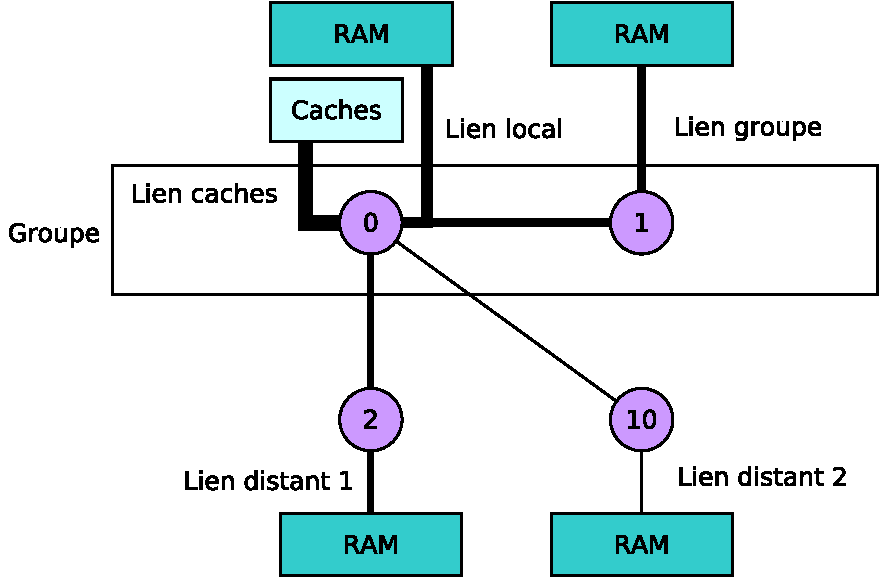
\includegraphics[width=\textwidth]{topo-idchire}
  \caption{Topologie schématique vu du nœud 0}\label{fig:contribs:machines:idchire:topo-liens}
\end{figure}

L'interconnexion des nœuds NUMA est effectué à travers l'Intel \emph{Quick Path Interconnect} (QPI).
La topologie de la machine expose une hiérarchie à plusieurs niveaux, la Figure~\ref{fig:contribs:machines:idchire:topo-liens} présente la hiérarchie de la machine du point de vue du nœud 0.
Chaque nœud est d'abord associé à un autre nœud pour former un groupe. Ces groupes sont ensuite interconnectés entre eux et sont accessibles en deux rebonds maximum dans le système d'interconnexion.
Pour chaque nœud il y a 12 nœuds situés à un rebond, et 10 nœuds situés à deux rebonds.

\begin{figure}[t!]
  \centering
  \includegraphics[width=\textwidth]{heatmap_idchire_memcpy}
  \caption{Carte de la bande passante d'idchire}\label{fig:contribs:machines:idchire:heatmap}
\end{figure}

\begin{figure}[h!]
  \centering
  \includegraphics[width=0.9\textwidth]{link_saturation}
  \caption{Bande passante depuis le nœud 0, en fonction du nombre de threads effectuant une copie et du nœud destination}\label{fig:contribs:machines:idchire:saturation}
\end{figure}


La Figure~\ref{fig:contribs:machines:idchire:heatmap} présente la bande passante nœud à nœud en fonction de la source et de la destination, mesurée à l'aide d'une copie de tableau (|memcpy|) de 200 Mo.
Elle fait apparaître clairement une diagonale où la bande passante est significativement plus grande, illustrant le coût d'un accès mémoire local comparé à un accès distant.

Néanmoins cette simple <<carte>> ne suffit pas à caractériser complètement les temps d'accès aux nœuds NUMA, puisque qu'une seule communication ne va pas saturer la bande passante totale disponible, ni même illustrer l'impact de la contention.


\subsubsection{Mesure des liens}\label{sec:contribs:machines:idchire:liens}

En dehors de l'accès aux caches locaux, il y a 4 liens à quantifier, identifiés sur la Figure~\ref{fig:contribs:machines:idchire:topo-liens}.
Afin de mesurer chacun des liens, nous avons défini des scénarios spécifiques que nous avons exécuté via \outil~: pour un nœud NUMA source donné (ici 0), nous avons alloué et initialisé deux tableaux de 200 Mo. Le premier sur le nœud source, et le second sur le nœud local. Nous avons ensuite effectué une copie du tableau source vers le tableau local (via |memcpy|) et mesuré le temps de l'opération.
Pour chaque type de nœud source (même nœud, distant sur le même groupe, distant via un rebond, distant via deux rebonds), nous avons effectués de une à huit copies simultanées.


La Figure~\ref{fig:contribs:machines:idchire:saturation} regroupe les résultats de la bande passante cumulée en fonction de nombre de copies simultanées ayant lieu, et en fonction du nœud cible.
On constate que la bande passante maximum du lien local atteint 12.2 Go/s, et qu'il commence à saturer lorsque plus de la moitié des cœurs sont utilisés.
Le lien groupe plafonne à 5.6 Go/s, le lien distant 1 plafonne à 5.1 Go/s, et le lien distant 2 à 4.8 Go/s.


\begin{todo}
  Figure saturation output du noeud
\end{todo}


\subsection{brunch}\label{sec:contribs:machines:brunch}

Cette machine est équipée de 4 processeurs Intel(R) Xeon(R) CPU E7-8890 v4 (Broadwell), cadencés à 2.2 GHz.

Chacun de ce processeurs est associé à 378 Go de RAM pour former un nœud NUMA, ils disposent de 24 cœurs physiques partageant 60 Mo de cache L3 (20-ways associatifs).
Chacun des cœur à accès à 32 Ko de cache L1 (données) et 256 Ko de cache L2.

La machine entière dispose donc de 96 cœurs physiques, et de 1.5 To de RAM.
Les processeurs Broadwell disposent d'instructions FMA~\footnote{\emph{Fused Multiply-Add}, permettant d'effectuer une addition et une multiplication en une étape}, permettant d'effectuer 8 additions et multiplications de nombres flottant à double précision en un cycle, portant le pic de performance théorique de la machine à 3.3 TFLOPs.


\subsubsection{Topologie}

L'interconnexion des nœuds NUMA est effectué à travers l'Intel \emph{Quick Path Interconnect} (QPI).
Contrairement à idchire, la topologie de la machine est relativement plate~: les nœuds sont directement connectés les uns aux autres, et seule la notion d'accès distant ou local permet de distinguer une hiérarchie.

\begin{figure}[h]
  \centering
  \includegraphics[width=\textwidth]{heatmap_brunch}
  \caption{Carte de la bande passante de brunch}\label{fig:contribs:machines:brunch:heatmap}
\end{figure}

La Figure~\ref{fig:contribs:machines:brunch:heatmap} présente la bande passante nœud à nœud en fonction de la source et de la destination, mesurée à l'aide d'une copie de tableau (|memcpy|) de 200 Mo.
Bien qu'une diagonale se dégage clairement, la différence entre accès local et accès distant n'est de l'ordre que de 10\%, comme en témoigne l'échelle de couleur sur la figure.

\subsubsection{Mesure des liens}

De même que pour idchire, nous avons effectué des observations complémentaires pour caractériser plus précisément les liens locaux et distant, afin de déterminer leur saturation.

\begin{todo}
  TODO, faire le graphe et la conclusion
\end{todo}


\section{Une étude de cas : Cholesky}\label{sec:contribs:apps:cholesky}

Afin de mettre en application nos analyses nous avons choisi comme cas d'étude une application d'algèbre linéaire très étudiée et bien connue : la factorisation de Cholesky.
Une manière standard de paralléliser les applications d'algèbre linéaire est de découper le problème en l'appliquant à différentes sous parties (ou \emph{blocs}) des matrices.

Nous allons étudier en détails l'algorithme de Cholesky par blocs tel qu'implémenté dans PLASMA~\cite{Kurzak2013}, dont nous donnons le code dans le listing~\ref{lst:contribs:apps:cholesky-block-plasma}.
Nous allons voir quelles sont ses parties critiques et leurs comportements, et nous allons également voir comment nous avons pu améliorer son exécution.

\begin{figure}[h]
\begin{lstlisting}[language=c++,caption=Algorithme de Cholesky par bloc tel qu'exprimé dans PLASMA,label=lst:contribs:apps:cholesky-block-plasma]
for (int k = 0; k < n_blocs; k++) {
  DPOTRF(A(k, k));

  for (int m = k+1; m < n_blocs; m++) {
    DTRSM(A(k, k), A(k, m));
  }

  for (int m = k+1; m < n_blocs; m++) {
    DSYRK(A(k, m), A(k, k));

    for (int n = k+1; n < m; n++) {
      DGEMM(A(k, n), A(k, m), A(n, m));
    }
  }
}
\end{lstlisting}
\end{figure}


\subsection{Description générale}

La factorisation de Cholesky a pour but de résoudre l'équation suivante :

$$ A = L*L^T$$

Où $A$ est une matrice symétrique définie positive à coefficients réels, et $L$ est l'inconnue, une matrice triangulaire inférieure.

Pour paralléliser la résolution de cette équation, nous allons découper la matrice $A$ par bloc, et appliquer un algorithme de Cholesky par bloc.
Nous pouvons donc caractériser une factorisation de Cholesky par sa taille de bloc et sa largeur en nombre de blocs.

L'algorithme de résolution par bloc repose sur quatre algorithmes basiques d'algèbre linéaire tirés des \emph{BLAS} - \emph{Basic Linear Algebra Subprograms} - décrits ci-dessous~:


\paragraph{\potrfcolor{POTRF(A)}}

Ce noyau effectue la factorisation de Cholesky de base sur une matrice symétrique définie positive $A$.

\paragraph{\trsmcolor{TRSM(A, B)}}

Ce noyau résoud l'équation suivante~: $A*X = B$, où $A$ est une matrice triangulaire, et $B$ une matrice générique. $B$ est écrasée par la matrice solution $X$.

\paragraph{\syrkcolor{SYRK(A, C)}}

Ce noyau effectue l'opération suivante~: $C := A*A^t + C$, où $A$ est une matrice générique, et $C$ est une matrice symétrique.

\paragraph{\gemmcolor{GEMM(A, B, C)}}

Ce noyau effectue une multiplication de matrices génériques, définie de la manière suivante~: $C := A*B + C$, où $A$, $B$, et $C$ sont des matrices génériques.

\begin{figure}[h]
  \centering
  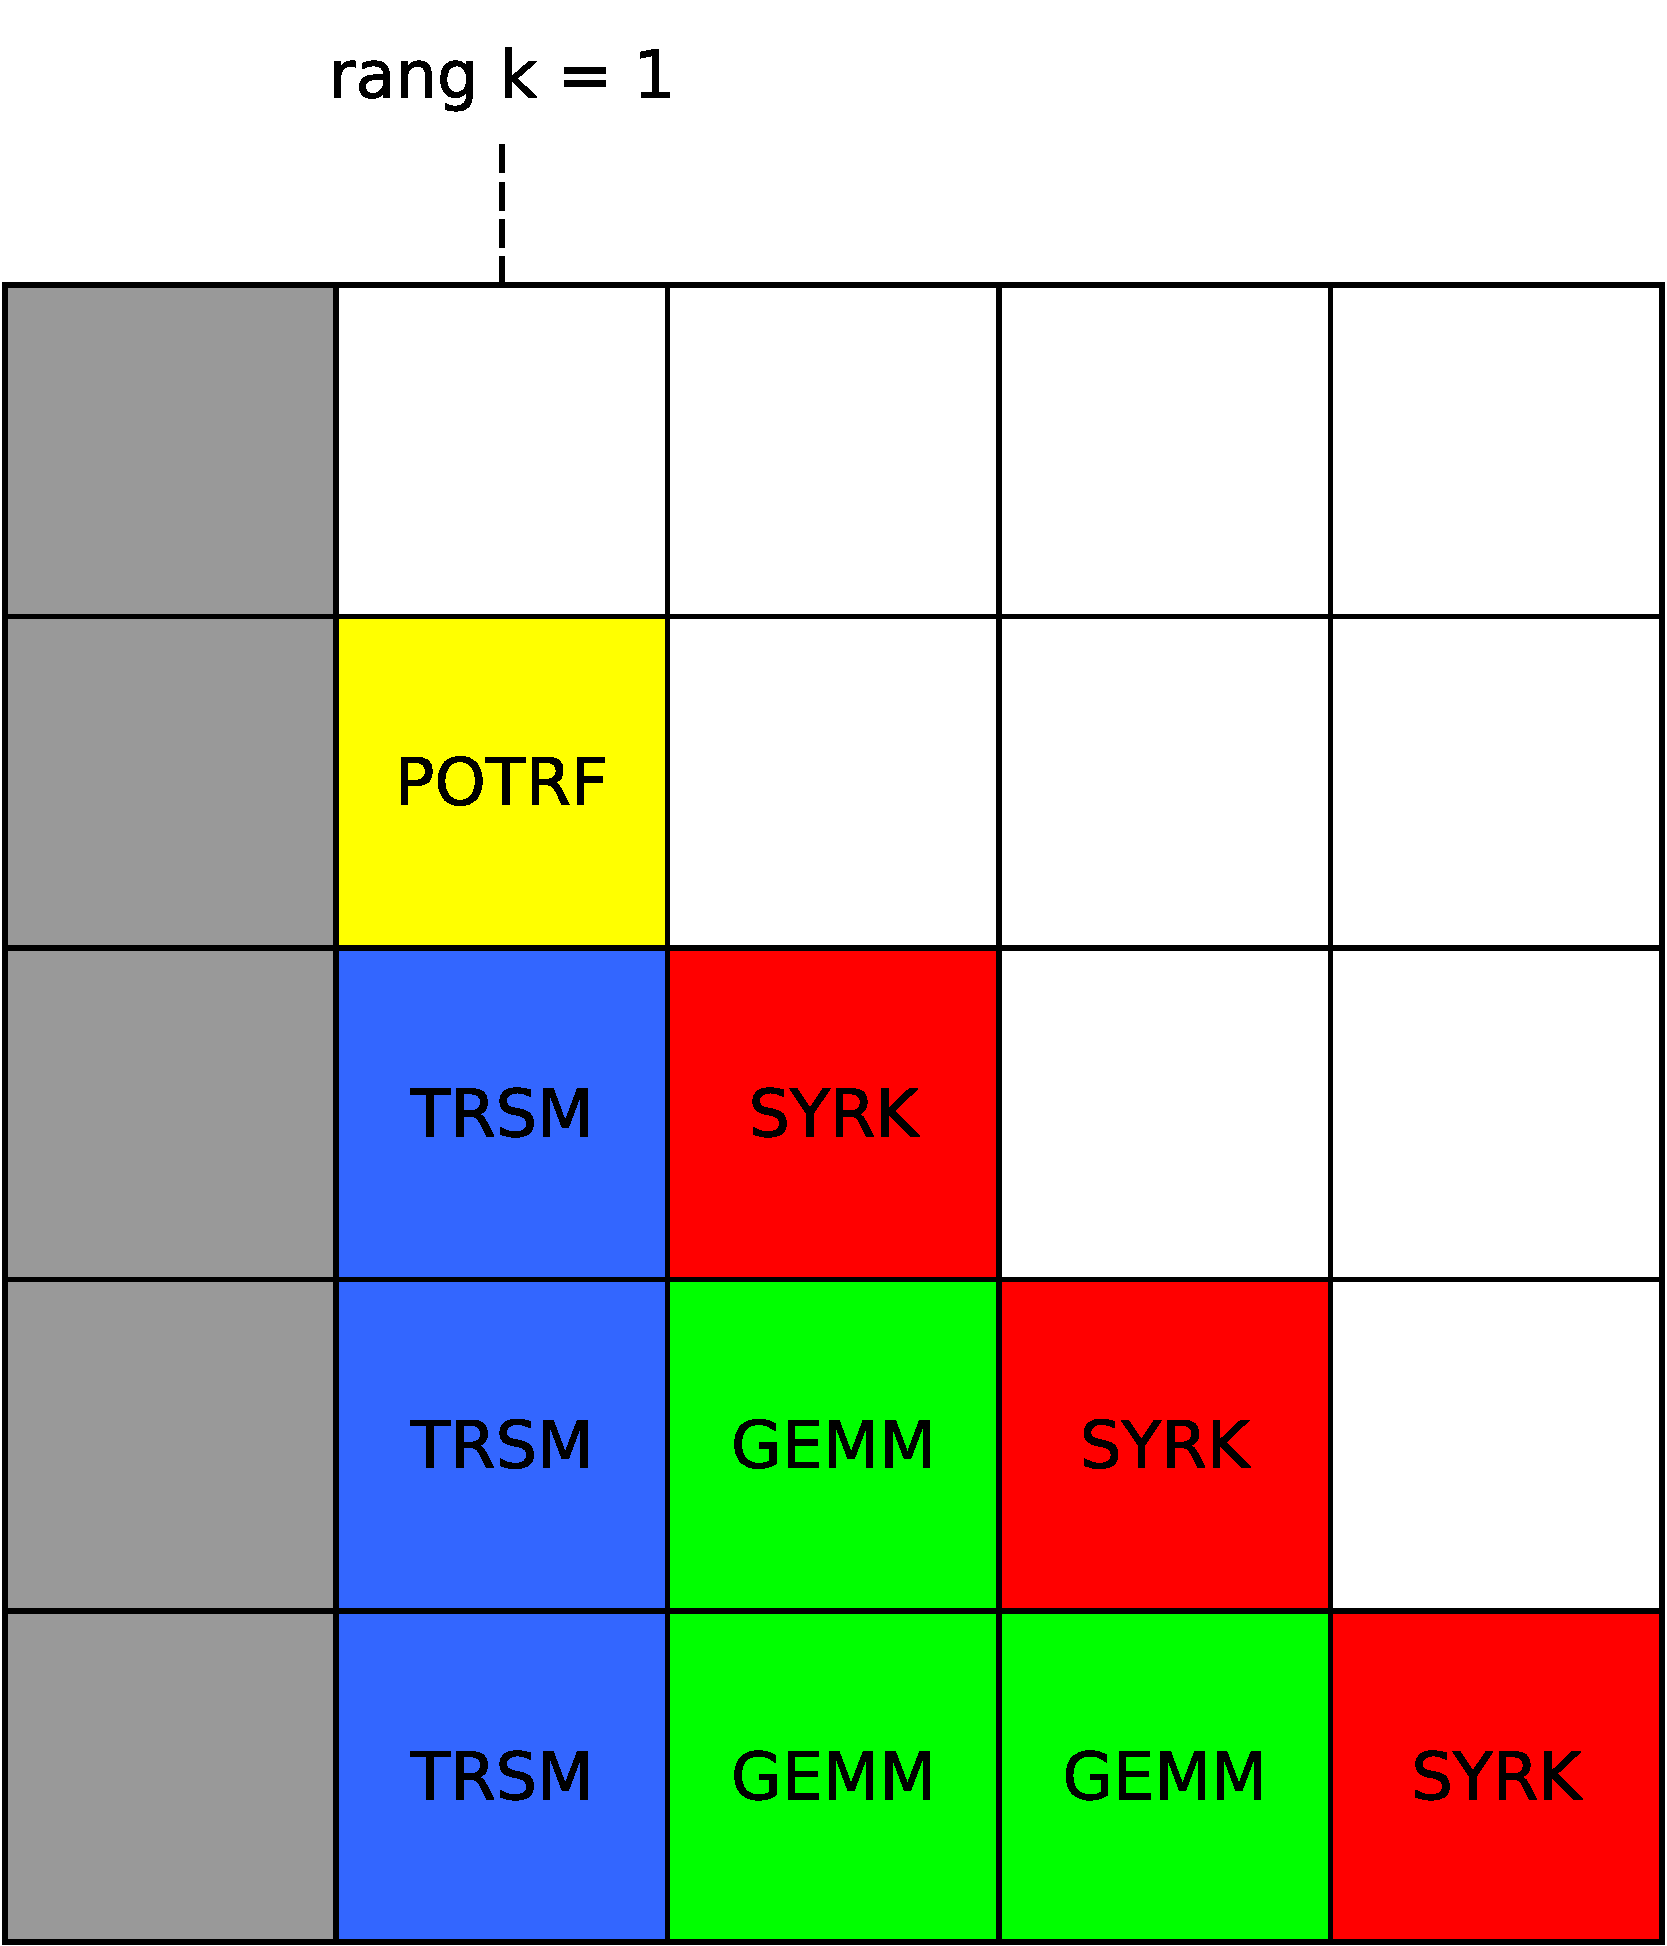
\includegraphics[width=0.6\textwidth]{cholesky-rank-update}
  \caption{Itération du rang k de la factorisation de Cholesky}\label{fig:contribs:apps:cholesky:rank-update}
\end{figure}

Pour permettre de mieux représenter l'algorithme du listing~\ref{lst:contribs:apps:cholesky-block-plasma}, les opérations se produisant sur chaque bloc de la matrice au rang |k| sont illustrées sur la figure~\ref{fig:contribs:apps:cholesky:rank-update}


À chaque itération, un \potrf est d'abord effectué sur le bloc diagonal de l'itération. Les blocs de la colonne sont ensuite mis à jour via des \trsm, à la suite desquels les autres blocs restant peuvent être mis à jour par des \gemm (ou \syrk pour les blocs diagonaux).
Le parallélisme de l'algorithme est donc principalement libéré par les \potrf ainsi que les \trsm.
Cela peut être illustré par la Figure~\ref{fig:contribs:apps:cholesky:dag-5}, qui donne le graphe de dépendances d'une factorisation de Cholesky de largeur 5.

\begin{figure}[h]
  \centering
  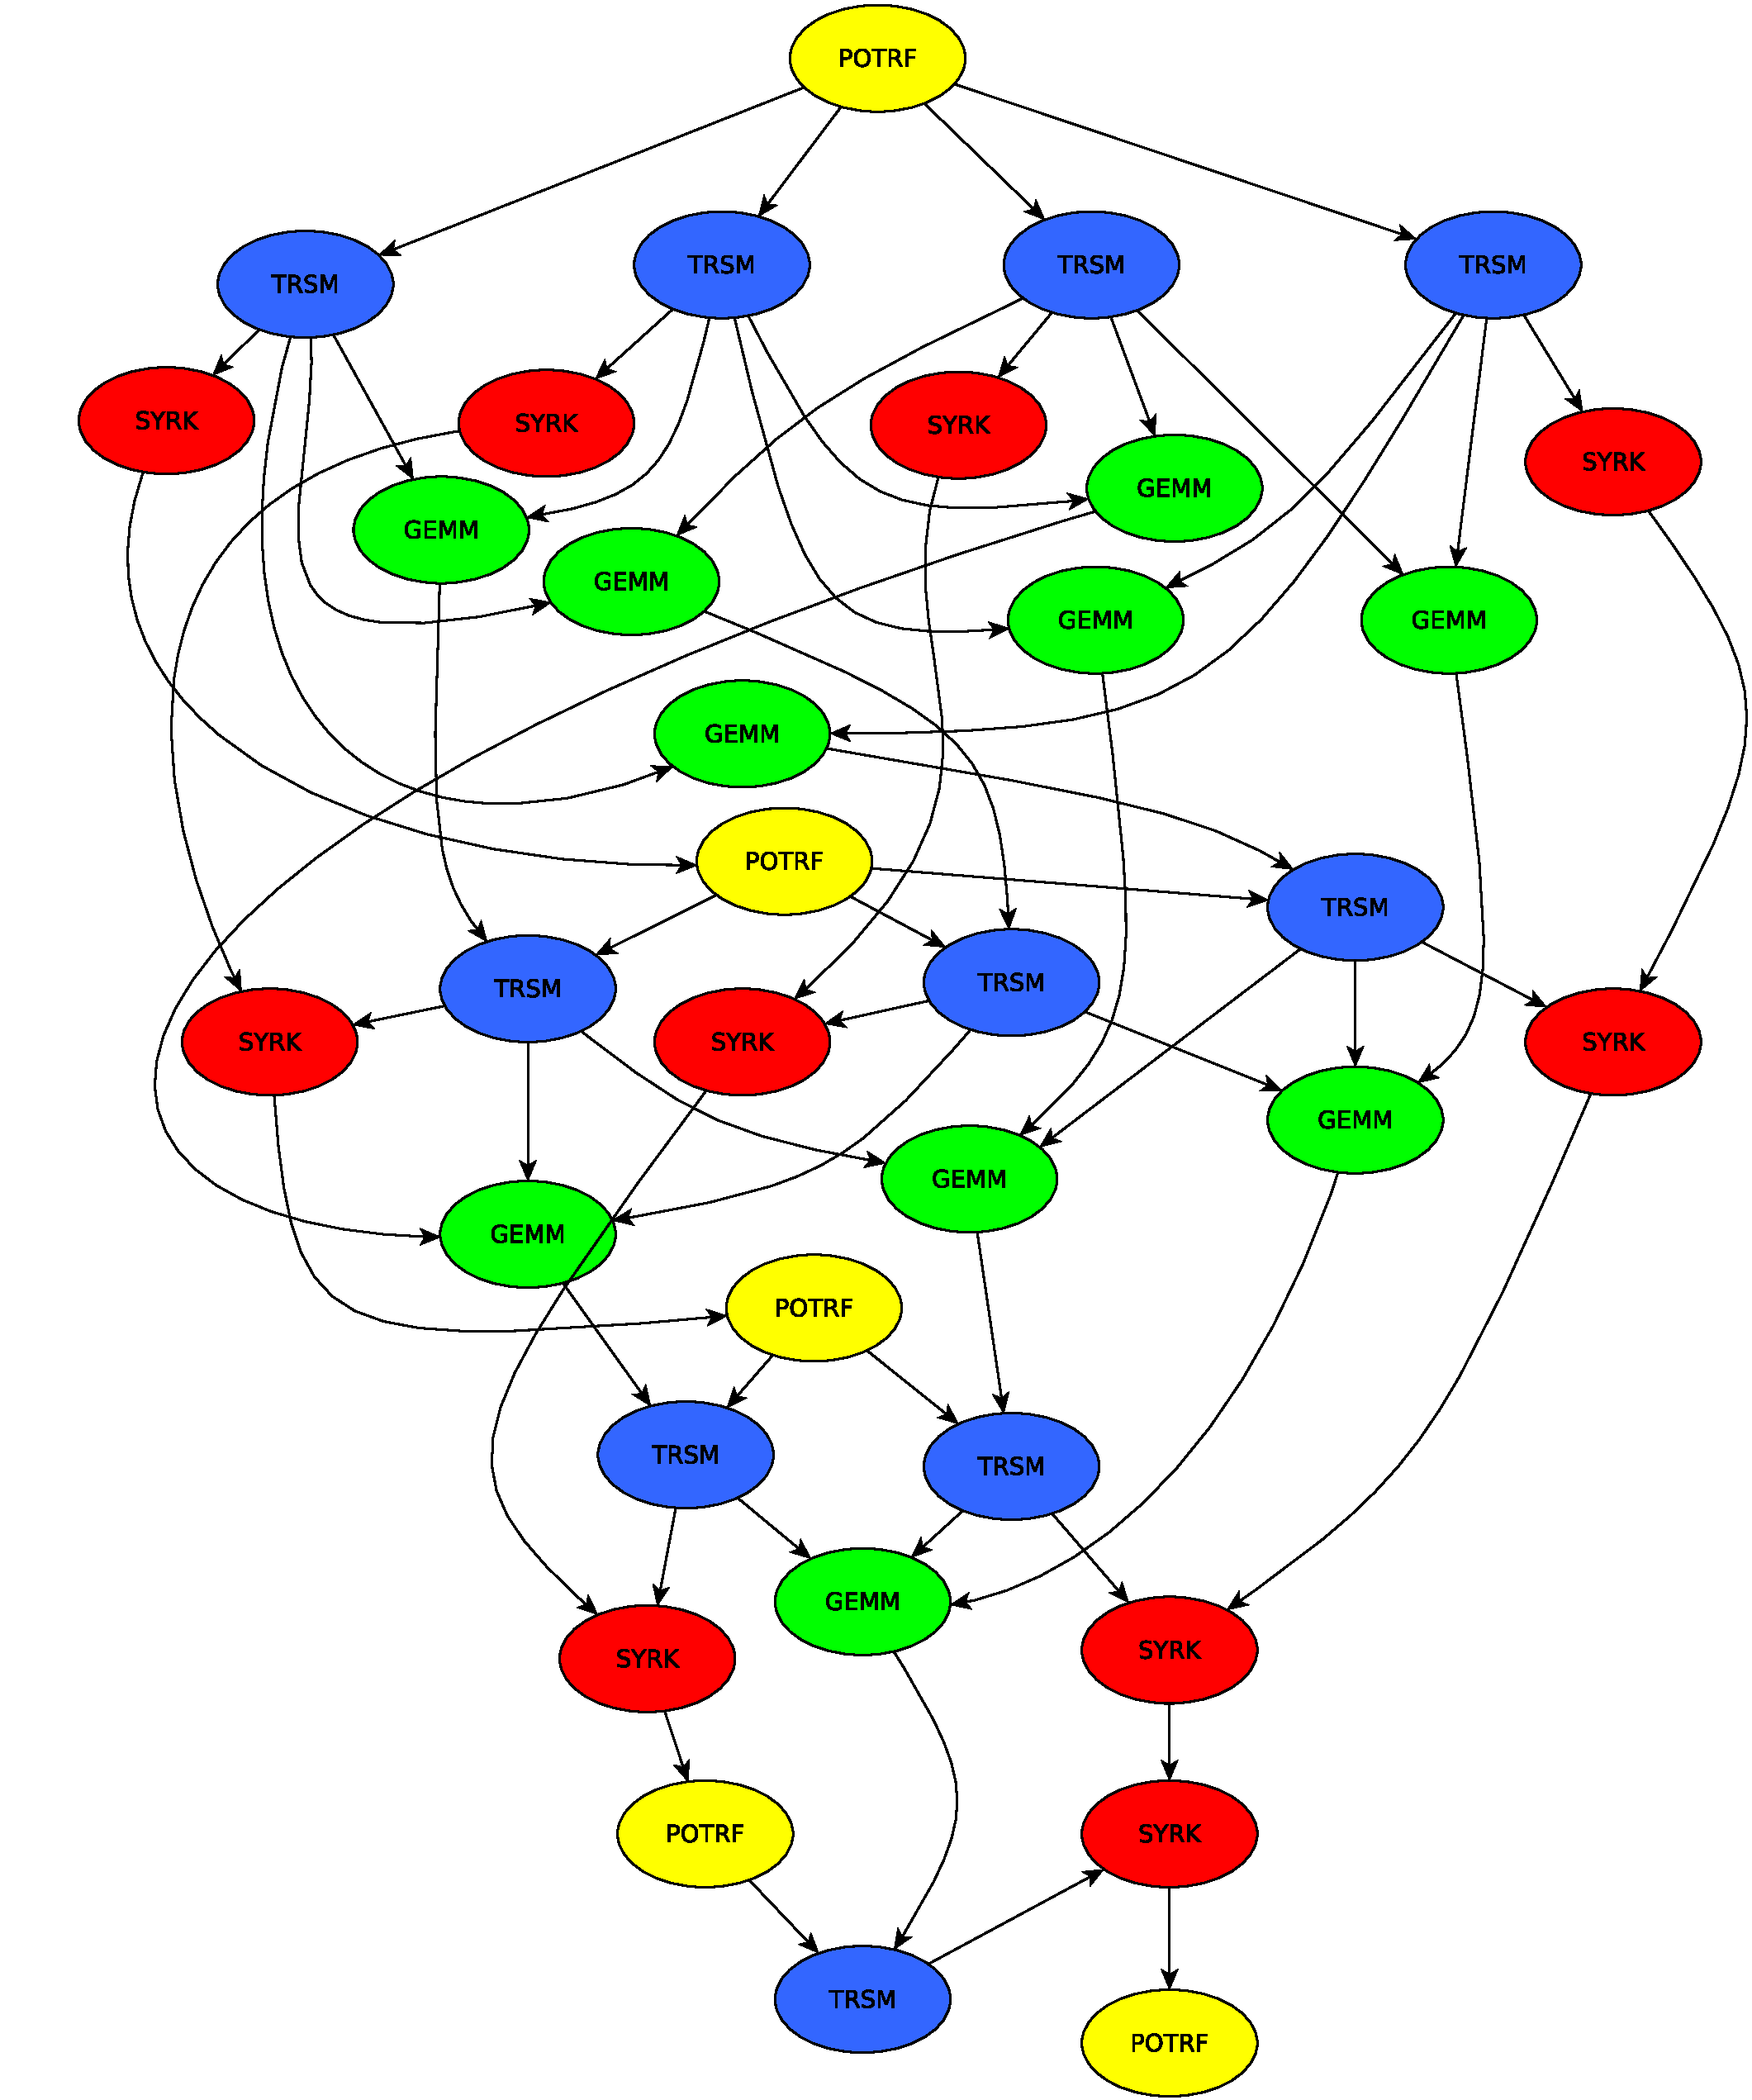
\includegraphics[width=0.7\textwidth]{cholesky-dag-5}
  \caption{DAG d'un Cholesky de largeur 5}\label{fig:contribs:apps:cholesky:dag-5}
\end{figure}

Le nombre de tâches créées pour une largeur de matrice $L$ (en nombre de blocs), le nombre d'opérations arithmétiques flottantes (ou \emph{flops}) en fonction de la taille de bloc $N$, ainsi que l'intensité opérationnelle\footnote{Définie par $\frac{Flops}{bytes}$} sont résumés dans la table~\ref{tab:contribs:apps:cholesky:kernels-info}.


\begin{table}[h!]
\def\arraystretch{1.5}
\centering
\begin{tabular}{|c||c|c|c|}\hline
  Noyau & \makecell{Nombre pour une\\largeur de matrice $L$} & \makecell{Flops pour une\\ taille de bloc $N$~\cite{LAWN41}} & \makecell{Intensité\\Opérationnelle} \\ \hline
  \potrf & $L$ & $\frac{N^3}{3} + \frac{N^2}{2} + \frac{N}{6}$ & $\frac{N}{24} + o(N)$ \\ \hline
  \trsm & $\frac{L*(L-1)}{2}$ & $N^3$ & $\frac{N}{8} + o(N)$ \\ \hline
  \syrk & $\frac{L*(L-1)}{2}$ & $N^2*(N+1)$ & $\frac{N}{8} +o(N)$ \\ \hline
  \gemm & $\frac{L^3}{6} - \frac{L^2}{2} + \frac{L}{3} + 1$ & $2*N^3$ & $\frac{N}{4} +o(N)$ \\ \hline
%$\sum_{k=1}^{n}\frac{(k-1)*(k-2)}{2}$
%simplifié via wolframalpha
\end{tabular}
\caption{Nombre et complexité des différents noyaux}\label{tab:contribs:apps:cholesky:kernels-info}
\end{table}

Les \gemm sont donc très largement majoritaires dans l'algorithme quand la largeur de la matrice augmente.
En revanche en terme de Flops et d'intensité opérationnelle, on peut constater que tous les noyaux présentent des chiffres d'un ordre de grandeur équivalent.


\subsection{Observations préliminaires et limites}\label{sec:contribs:apps:cholesky:observations}

Cette section et les suivantes montrent des évaluations reposant sur une bibliothèque BLAS, sauf indication contraire, la version utilisée est OpenBLAS 2.19.
La figure~\ref{fig:context:granularity} a montré qu'on pouvait observer l'impact de certains paramètres, tels que la taille de bloc ou le support exécutif, sur les performances globales.

Certains supports exécutifs tels que Kaapi, StarPU, OpenStream, ou encore OmpSs permettent d'aller plus loin via un système de traces, permettant d'observer certaines caractéristiques de tâches particulières.

\begin{figure}[t!]
  \centering
  \includegraphics[width=\textwidth]{graph_evolution_cholesky_8192_224}
  \caption{Évolution des performances de Cholesky avec libKOMP, pour une taille de matrice de 8192 et une taille de bloc de 224}\label{fig:contribs:apps:cholesky:overview-8192-224}
\end{figure}

Pour illustrer cela, prenons un exemple d'évolution des performances de Cholesky en fonction du nombre de cœurs utilisés, montré sur la figure~\ref{fig:contribs:apps:cholesky:overview-8192-224}. Dans cet exemple la taille de matrice est de 8192, la taille de bloc de 224, et le support exécutif utilisé est libKOMP, sans aucune extension relatives à nos travaux sur l'affinité des données, que nous présentons dans le chapitre~\ref{chap:contrib:openmp}.

En activant le support des traces, on peut avoir plus de détails sur l'exécution individuelle de chacune des tâches.

\begin{figure}[h!]
  \centering
  \includegraphics[width=\textwidth]{graph_distrib_overview_8192_224}
  \caption{Distribution des différents noyaux en fonction du nombre de cœurs}\label{fig:contribs:apps:cholesky:distrib-overview-8192-224}
\end{figure}

La figure~\ref{fig:contribs:apps:cholesky:distrib-overview-8192-224} montre, pour chaque type de tâche (ou \emph{noyau}), la répartition du temps d'exécution (en cycles) en fonction du nombre de cœurs.

On constate deux types de répartitions~:
\begin{itemize}
  \item Une distribution relativement restreinte des cycles de chaque noyau, typiquement observée pour 16 cœurs.
    La distribution peut avoir plusieurs pics~: pour \gemm sur 16 cœurs par exemple.
    Cela pourrait être expliqué par le nombre de cas possibles pour le placement des blocs de données manipulés par le noyau~: avec 16 cœurs il y a 2 nœuds impliqués, et donc 4 cas pour la position des blocs (3 locaux, 2 locaux, 1 local, 3 distants), ce qui pourrait correspondre aux 4 niveaux de performances observés.
  \item Une distribution relativement large, typiquement observée pour un grand nombre de cœur. Pour un \gemm sur 192 cœurs, le nombre de cycles nécessaires pour l'exécution peut varier du simple au double !
\end{itemize}

Nous souhaiterions identifier d'où vient cette évolution dans la distribution, afin d'éventuellement réussir à la corriger en limitant sa largeur.

Malheureusement il n'existait pas, à notre connaissance, d'outil permettant d'isoler une (ou plusieurs) tâches d'une application, et permettant de changer certains paramètres prédéfinis pouvant avoir un impact sur le temps d'exécution de la tâche.
Nous avons donc utilisé \outil dans le but de comprendre et d'analyser plus en profondeur nos observations préliminaires.

\subsection{Caractérisation détaillée des noyaux via \outil}\label{sec:contribs:apps:cholesky:carton}

L'objectif de cette section est de décrire le processus expérimental nous ayant permis d'analyser et comprendre le comportement des quatre noyaux de Cholesky~: \potrf, \trsm, \syrk, \gemm, qui a finalement abouti à des améliorations du support exécutif.
Nous allons donc aborder d'une part les types de scénarios exécutés via \outil, puis illustrer les résultats que nous avons obtenus avec des exemples significatifs.

\subsubsection{Description des scénarios}\label{sec:contribs:apps:cholesky:scenario}

Afin d'étudier le comportement de chaque noyau impliqué dans Cholesky, nous avons défini des scénarios au cours desquels les noyaux sont exécutés avec un contrôle sur les conditions d'exécution.

Pour un noyau donné (parmi \potrf, \trsm, \syrk, \gemm), le scénario de base est le suivant :
\begin{itemize}
  \item Allocation et initialisation des données sur un nœud précis pour une taille de bloc donnée.
  \item Exécution d'un certain nombre de répétitions du noyau choisi (par défaut 50) sur ces données, en plaçant le thread de calcul soit sur un cœur du même nœud que les données, soit sur un cœur distant.
  \item Observation de la performance en FLOPS.
\end{itemize}

Ce scénario de base est donné en entier dans l'annexe~\ref{chap:annexe:tool:dgemm-base}, pour l'exécution d'un \gemm local de taille 256.

Pour évaluer le comportement des noyaux en fonction de la charge de la machine, nous avons créé des scénarios exécutant simultanément plusieurs noyaux sur des données complètement indépendantes, et où le démarrage de l'exécution des noyaux est synchronisé.
L'annexe~\ref{chap:annexe:tool:dgemm} illustre l'un de ces scénarios, qui permet d'exécuter 8 \gemm en parallèle, sur des données locales complètement indépendantes, avec une taille de matrice de 256.

Il y a plusieurs paramètres que l'on peut faire varier pour changer les conditions d'exécution~:
\begin{itemize}
  \item Le nombre de noyaux s'exécutant simultanément~;
  \item L'utilisation de données distantes ou locales~;
  \item La taille du bloc sur lequel appliquer le noyau.
\end{itemize}

Les trois sections suivantes décrivent l'impact des changements de ces paramètres, et illustrent certaines caractéristiques des machines utilisées qui donnent des opportunités pour de possibles améliorations du support exécutif.

\subsubsection{Exécutions simultanées}

\begin{figure}[ht]
  \centering
  \includegraphics[width=0.95\textwidth]{kernel_256_local_idchire}
  \caption{Performances des noyaux (B=256) avec données locales sur idchire}\label{fig:contribs:apps:cholesky:perf-256-local}
\end{figure}

Afin d'évaluer l'impact de la charge de la machine, nous avons lancé des scénarios avec un nombre variable d'exécutions simultanées de chacun des noyaux.
Pour le remplissage de la machine, nous avons placé les exécutions linéairement sur la machine, remplissant progressivement un nœud après l'autre.

La figure~\ref{fig:contribs:apps:cholesky:perf-256-local} montre la performance moyenne (en GFlops) de chaque noyau, en fonction du nombre de cœurs exécutant simultanément des noyaux.
Par exemple pour déterminer le point d'abscisse 144 sur la figure pour un \gemm, nous avons exécuté 50 répétitions de \gemm sur chacun des 144 premiers cœurs de la machine idchire (remplissant donc les 18 premiers nœuds), de manière indépendante et simultanée.
La performance moyenne pour ce point est obtenue en faisant la moyenne des performances sur l'ensemble des exécutions.
Pour ce cas la taille de bloc a été fixée à 256, avec les données allouées et initialisées localement.

Pour une taille de bloc de 256, la quantité maximale de données utilisée par l'un des noyaux (\gemm) est de 256*256*8*3 = 1.5 Mo. La taille du cache L2 étant de 256 Ko, le jeu de données ne tient pas dans ce cache. Mais avec un nœud de 8 cœurs exécutant 8 exécutions concurrentes, la quantité totale de données utilisée serait au pire de 12.58 Mo, soit environ 50\% des 20Mo de cache L3 disponible.
On pourrait donc s'attendre à ce que la performance moyenne des noyaux ne soit impactée que par des effets locaux aux nœuds.

Néanmoins les courbes montrent clairement une dégradation des performances de chaque noyaux lorsque la charge de la machine augmente.
Ce comportement a également été observé pour d'autres tailles de blocs. Sur brunch le comportement a été également observé, avec néanmoins une dégradation moindre.

\begin{todo}
  faire la mesure via hubstat pour confirmer ou infirmer l'hypothèse de la cohérence.

  %https://www.researchgate.net/profile/Daniel_Molka/publication/315703632_Performance_Analysis_of_Complex_Shared_Memory_Systems/links/58dd3cf292851cd2d3d9d5d3/Performance-Analysis-of-Complex-Shared-Memory-Systems.pdf
  %https://pdfs.semanticscholar.org/67cf/1189c859d66bac309f9438df434fb651f97a.pdf
  % sandy bridge : https://tu-dresden.de/zih/forschung/ressourcen/dateien/abgeschlossene-projekte/benchit/2014_MSPC_authors_version.pdf?lang=en
  % haswell : https://pdfs.semanticscholar.org/67cf/1189c859d66bac309f9438df434fb651f97a.pdf
\end{todo}

\subsubsection{Impact de la localité des accès}\label{sec:contribs:apps:cholesky:locality}

Les expériences de bande passante dans la section précédente ont montrées des différences significatives dans les temps d'accès à la mémoire locale et distante.
Nous avons donc déroulé des scénarios avec des noyaux utilisant des données distantes ou des données locales afin de pouvoir les comparer, et éventuellement déceler des comportements typiques.
Lorsque les données sont dites <<locales>>, l'ensemble des données est allouée sur le nœud local. Lorsque les données sont dites <<distantes>>, l'ensemble des données est alloué sur le nœud suivant (numériquement) dans la hiérarchie de la machine.

\begin{figure}[t!]
  \centering
  \includegraphics[width=0.95\textwidth]{kernel_512_remote_idchire}
  \caption{Performances GEMM, POTRF (B=512) avec données distantes sur \emph{idchire}}\label{fig:contribs:apps:cholesky:perf-512-remote-idchire}
\end{figure}
\begin{figure}[h!]
  \centering
  \includegraphics[width=0.95\textwidth]{kernel_512_remote_brunch}
  \caption{Performances GEMM, POTRF (B=512) avec données distantes sur \emph{brunch}}\label{fig:contribs:apps:cholesky:perf-512-remote-brunch}
\end{figure}

Les figures~\ref{fig:contribs:apps:cholesky:perf-512-remote-idchire} et~\ref{fig:contribs:apps:cholesky:perf-512-remote-brunch} illustrent les performances de deux noyaux, \gemm et \potrf, exécutés en concurrence sur des blocs de 512, en fonction du type d'accès, sur idchire et brunch, respectivement.

Avec une telle taille de bloc, l'ensemble des données pour tous les \potrf tient dans le cache L3, mais ce n'est pas le cas pour \gemm.
Pour les \potrf la dégradation de performances est moindre : les données tiennent dans le cache L3, il y a donc un coût pour rapatrier les données, mais une fois les données dans le cache L3 il n'y a plus besoin de faire d'accès distants.

Pour les \gemm, une utilisation de seulement quelques cœurs ne montre pas une différence de performances flagrante, en revanche le lien en sortie de nœud arrive assez vite à saturation (voir section~\ref{sec:contribs:machines:idchire:liens}), ce qui entraine une dégradation massive de performances.
À la fois pour idchire et brunch, on peut observer l'impact de la bande passante sur les performances~: les exécutions sont placées de manière à remplir progressivement les différents nœuds de la machine, et on peut observer que les courbes sont en dent de scie avec une période égale à la taille des nœuds sur chaque machine (8 sur idchire, 24 sur brunch).

Cela devient évident lorsqu'on regarde plus en détail le passage d'un nœud à un autre.
Sur la figure~\ref{fig:contribs:apps:cholesky:perf-512-remote-brunch}, la courbe pour les \gemm distants remonte progressivement entre 24 et 36 cœurs utilisés~: le fait de faire la moyenne des noyaux sur l'ensemble des cœurs cache légèrement le phénomène de saturation du lien.
En revanche ce phénomène devient évident lorsque l'on affiche la moyenne du temps d'exécution par cœurs pour certains des points de la courbe, comme illustré sur la figure~\ref{fig:contribs:apps:cholesky:distrib-load-512}.

\begin{figure}[ht]
  \centering
  \includegraphics[width=0.95\textwidth]{illustration_load_avg}
  \caption{Distribution des performances de chaque noyau (Bloc = 512), en fonction du nombre total d'exécutions concurrentes, sur brunch.}\label{fig:contribs:apps:cholesky:distrib-load-512}
\end{figure}

Le premier panneau montre la distribution des \gemm et des \potrf pour une exécution sur 24 cœurs concurrents situés sur le même nœud.
Cette distribution montre un unique pic bien défini pour chaque noyau (environ 12.5 GFlops pour \potrf, et 16.5 pour \gemm).
En revanche le passage à 26 cœurs (avec donc 2 cœurs situés seuls sur un autre nœud), montre une distribution avec deux pics~: un pic important correspondant au 24 premiers cœurs, et un second pic plus petit, montrant des performances beaucoup plus grandes, pour les 2 cœurs situé sur l'autre nœud.
Les autres panneaux montrent l'évolution de ces pics pour arriver au panneau 48, où les deux nœuds sont complètement utilisés.

%Note : Ici il y a aussi deux pics sur le panneau 48. Cela doit venir de la manière dont j'ai initialisé les accès distants : le premier nœud utilise des données du deuxième nœud, qui utilise des données du troisième nœud. Donc en pratique les liens du deuxième nœuds sont plus utilisés que ceux du premier : il doit donc un peu peiner à fournir les données nécessaires au premier nœud, ce qui expliquerait pourquoi il y a deux groupes de perf.


L'impact de la localité des données est majeur dans le cas où le jeu de données manipulé par l'ensemble des cœurs ne tient pas dans les caches L3.
Étant donné que la plus grande proportion des noyaux de Cholesky manipule 2 ou 3 blocs, la dégradation de performance devrait être importante lorsque la taille de bloc dépasse environ 320.

% Note : à la fois sur brunch et idchire, chaque cœur peut utiliser environ 2.5Mo de cache L3



\subsubsection{Impact de la taille de bloc}

La figure~\ref{fig:contribs:apps:cholesky:perf-multiple-bs-idchire} montre la performance des \gemm et \potrf sur idchire en fonction de la taille de bloc et du nombre de cœurs utilisés (tous les accès sont locaux).

\begin{figure}[ht]
  \centering
  \includegraphics[width=0.95\textwidth]{kernels_multiple_bs_local_idchire}
  \caption{Performances des noyaux avec données locales sur idchire}\label{fig:contribs:apps:cholesky:perf-multiple-bs-idchire}
\end{figure}

La taille de bloc n'a pas d'impact significatif sur le phénomène observé précédemment de dégradation des performances.
Elle a bien un impact sur le niveau de performance globale de chaque noyau (qui dépend de l'implémentation des BLAS), mais le comportement général de chaque noyau reste le même.

Cette conclusion est similaire lors d'un placement distant des données.


\subsubsection{Impact de la bibliothèque BLAS}

Pour comparer l'impact potentiel de la bibliothèque implémentant les BLAS, nous avons configuré \outil pour qu'il utilise soit OpenBLAS (2.19), Intel MKL (11.3), ou ATLAS (3.10.3).
La figure~\ref{fig:contribs:apps:cholesky:perf-blas} montre la performance des \gemm et \potrf sur \emph{brunch}, pour une taille de bloc de 256 avec des données locales, en fonction de la bibliothèque BLAS utilisée.

\begin{figure}[ht]
  \centering
  \includegraphics[width=0.98\textwidth]{comparaison_atlas_openblas_mkl_256_local}
  \caption{Comparaison des bibliothèques BLAS sur \emph{brunch}, données locales, taille de bloc = 256}\label{fig:contribs:apps:cholesky:perf-blas}
\end{figure}

Bien qu'on puisse constater une différence de performance brute, il y a dans tous les cas une baisse (relativement faible) des performances avec l'augmentation du nombre d'exécution concurrentes, bien qu'elles soient toutes indépendantes.
Pour rappel sur \emph{brunch} chaque nœud dispose de 24 cœurs, et pour les \gemm on peut deviner une baisse sur ces 24 premiers cœurs, qui d'autant plus flagrante que la performance est grande.
Cela pourrait tout simplement s'expliquer par le fait qu'on atteint la limite de bande passante cumulée disponible sur le nœud local.
Pour les autres cas, l'impact de la bibliothèque semble concerner principalement le pic de performance de chaque noyau, sans différence majeure sur l'allure générale des courbes.

\subsection{Bilan et discussions}

La figure~\ref{fig:contribs:apps:cholesky:distrib-overview-8192-224} avait montrée, à l'aide des traces obtenues à partir d'une exécution, que nous pouvions observer une baisse et une dispersion des performances individuelles des noyaux de l'application Cholesky.
\outil nous a permis d'identifier principalement deux facteurs pouvant être à l'origine de ce phénomène~: tout d'abord une partie de la baisse de performance générale est due à la baisse de performance des noyaux qui accompagne l'augmentation de la charge de la machine.
\begin{todo}
  rappeler d'où ça vient quand c'est fait
\end{todo}
L'autre partie de cette baisse de performance, ainsi que la dispersion des temps d'exécution, peuvent être attribuées à une absence de contrôle de la localité des données au cours de l'application.



\bigskip
\bigskip

Le chapitre suivant est axé sur les différentes extensions que nous avons proposées dans le modèle de programmation et le support exécutif, afin d'essayer de mitiger le manque de localité des données.
En pratique les observations faites à travers \outil nous ont également servies à sélectionner des expériences et paramètres pertinents lors de l'évaluation des stratégies de vol de travail proposées avec la factorisation de Cholesky.
